%
%     hw2_bbordwell.tex
%     Baylee Bordwell (baylee.bordwell@colorado.edu)
%     Based on the template by Benjamin Brown (bpbrown@colorado.edu)
%     Aug 27, 2014
%
%     Problem set 2 for ASTR/ATOC 5540, Mathematical Methods, taught at
%     University of Colorado, Boulder, Fall 2014.
%
%

\documentclass[12pt, preprint]{aastex}
% formatting based on 2014 NASA ATP proposal with Jeff Oishi

%%%%%%begin preamble
\usepackage[hmargin=1in, vmargin=1in]{geometry} % Margins
\usepackage{hyperref}
\usepackage{url}
\usepackage{times}
\usepackage{natbib}
\usepackage{graphicx}
\usepackage{amsmath}
\usepackage{amsfonts}
\usepackage{amssymb}
\usepackage{pdfpages}
\usepackage{import}
% for code import
\usepackage{listings}
\usepackage{color}


\hypersetup{
     colorlinks   = true,
     citecolor     = gray,
     urlcolor       = blue
}

%% headers
\usepackage{fancyhdr}
\pagestyle{fancy}
\lhead{ASTR/ATOC 5540}
\chead{}
\rhead{name: Baylee Bordwell}
\lfoot{Problem Set 2}
\cfoot{\thepage}
\rfoot{Fall 2014}
% no hline under header
\renewcommand{\headrulewidth}{0pt}

\newcommand{\sol}{\ensuremath{\odot}}
\newcommand{\dedalus}{\href{http://dedalus-project.org}{Dedalus}}

% make lists compact
\usepackage{enumitem}
%\setlist{nosep}

%%%%%%end preamble


\begin{document}

\section*{Problem Set 2}
\section*{Numeric Linear Algebra with numpy}
\begin{enumerate}
\item The eigenvalues for the matrix A are:\newline
-1.9860+0$i$, -1.0209+2.5075$i$, -1.0209-2.5075$i$, 0.013846+2.0091$i$, 0.013846-2.0091$i$

One of the eigenvalues is purely real, and the four complex values are actually two pairs of the same value positive and negative.

\item 
\begin{figure}[!ht]
\centering
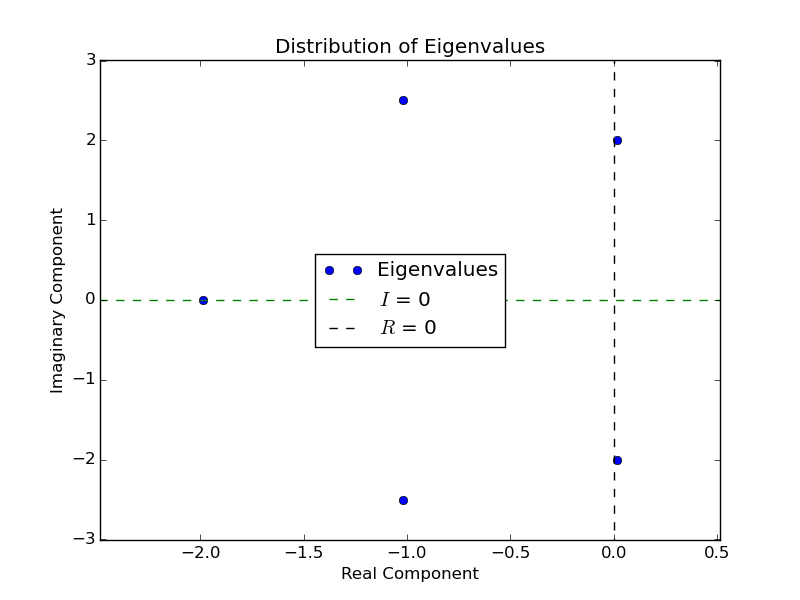
\includegraphics[width=5in]{hw2.png}
\end{figure}
\end{enumerate}


\section*{LU decompositions}
\begin{enumerate}
\item 
\[ A= \left( \begin{array}{ccc}
1 & -1 & 0 \\
-1 & 2 & -1 \\
0 & -1 & 2 \end{array} \right)  \indent
L= \left( \begin{array}{ccc}
1 & 0 & 0 \\
0 & 1 & 0 \\
0 & 0 & 1 \end{array} \right)\] 
\[ A'= \left( \begin{array}{ccc}
1 & -1 & 0 \\
0 & 1 & -1 \\
0 & -1 & 2 \end{array} \right)  \indent
L= \left( \begin{array}{ccc}
1 & 0 & 0 \\
-1 & 1 & 0 \\
0 & 0 & 1 \end{array} \right)\] 
\[ U = \left( \begin{array}{ccc}
1 & -1 & 0 \\
0 & 1 & -1 \\
0 & 0 & 1 \end{array} \right)  \indent
L= \left( \begin{array}{ccc}
1 & 0 & 0 \\
-1 & 1 & 0 \\
0 & -1 & 1 \end{array} \right)\] 

\begin{itemize}
\item \[L\textbf{y} = \textbf{b} =  \left[\begin{array}{l}
1  \\
0 \\
0 \end{array} \right], U\textbf{x} = \textbf{y}\] 
\[ \begin{array}{llr}
$L_{11}y_1 = b_1$ & $ y_1 = 1$ & \\
$L_{21}y_1+L_{22}y_2 = b_2$ & $y_2 = -1(-1)=1$ & $\rightarrow$\\
$L_{32}y_2+L_{33}y_3 = b_3$ & $y_3 = -1(-1)=1$ & \\
\end{array}
y= \left[ \begin{array}{c}
1 \\
1 \\
1 \end{array} \right] \]


\[ \begin{array}{llr}
$U_{11}x_1 + U_{12}x_2 = y_1$ & $x_1-x_2 = 1$ & \\
$U_{22}x_2 + U_{23}x_3 = y_2$ & $x_2-x_3 = 1$ & $\rightarrow$\\
$U_{33}x_3=y_3$ & $x_3 = 1 \text{ }\rightarrow \text{ } x_2 = 2, x_1 = 3$ & \\
\end{array}
x= \left[ \begin{array}{c}
3 \\
2 \\
1 \end{array} \right] \]

\item \[L\textbf{y} = \textbf{b} =  \left[\begin{array}{l}
0  \\
1 \\
0 \end{array} \right], U\textbf{x} = \textbf{y}\] 
\[ \begin{array}{llr}
$L_{11}y_1 = b_1$ & $ y_1 = 0$ & \\
$L_{21}y_1+L_{22}y_2 = b_2$ & $y_2 = 1$ & $\rightarrow$\\
$L_{32}y_2+L_{33}y_3 = b_3$ & $y_3 = -1(-1)=1$ & \\
\end{array}
y= \left[ \begin{array}{c}
0 \\
1 \\
1 \end{array} \right] \]


\[ \begin{array}{llr}
$U_{11}x_1 + U_{12}x_2 = y_1$ & $x_1-x_2 = 0$ & \\
$U_{22}x_2 + U_{23}x_3 = y_2$ & $x_2-x_3 = 1$ & $\rightarrow$\\
$U_{33}x_3=y_3$ & $x_3 = 1 \text{ }\rightarrow \text{ } x_2 = 2, x_1 = 2$ & \\
\end{array}
x= \left[ \begin{array}{c}
2 \\
2 \\
1 \end{array} \right] \]

\item \[L\textbf{y} = \textbf{b} =  \left[\begin{array}{l}
0  \\
0 \\
1 \end{array} \right], U\textbf{x} = \textbf{y}\] 
\[ \begin{array}{llr}
$L_{11}y_1 = b_1$ & $ y_1 = 0$ & \\
$L_{21}y_1+L_{22}y_2 = b_2$ & $y_2 = 0$ & $\rightarrow$\\
$L_{32}y_2+L_{33}y_3 = b_3$ & $y_3 = 1$ & \\
\end{array}
y= \left[ \begin{array}{c}
0 \\
0 \\
1 \end{array} \right] \]


\[ \begin{array}{llr}
$U_{11}x_1 + U_{12}x_2 = y_1$ & $x_1-x_2 = 0$ & \\
$U_{22}x_2 + U_{23}x_3 = y_2$ & $x_2-x_3 = 0$ & $\rightarrow$\\
$U_{33}x_3=y_3$ & $x_3 = 1 \text{ }\rightarrow \text{ } x_2 = 1, x_1 = 1$ & \\
\end{array}
x= \left[ \begin{array}{c}
1 \\
1 \\
1 \end{array} \right] \]
\end{itemize}

\item \verb|numpy.linalg.inv()| finds our 3 \textbf{x} to be the columnds of A$^{-1}$, which equals
\[ \left( \begin{array}{ccc}
 3 & 2 & 1 \\
 2 & 2 & 1 \\
 1 & 1 & 1 \\
\end{array} \right) \]
If this matrix is dotted with A using \verb|numpy.dot()|, the outcome is,
\[\[ \left( \begin{array}{ccc}
 1 & -1 & 0 \\
 -1 & 2 & -1 \\
 0 & -1 & 2 \\
\end{array} \right)
\left( \begin{array}{ccc}
 3 & 2 & 1 \\
 2 & 2 & 1 \\
 1 & 1 & 1 \\
\end{array} \right) =
 \left( \begin{array}{ccc}
 1 & 0 & 0 \\
 0 & 1 & 0 \\
 0 & 0 & 1 \\
\end{array} \right) \]\]
\end{enumerate}

\noindent Code involved in this assignment:
%
%     hw2_code.tex
%     Benjamin Brown (bpbrown@colorado.edu)
%     Aug 27, 2014
%
%     Problemset 2 for ASTR/ATOC 5540, Mathematical Methods, taught at
%     University of Colorado, Boulder, Fall 2014.
%
%     Python code importing block.
%


\definecolor{codegreen}{rgb}{0,0.6,0}
\definecolor{codegray}{rgb}{0.5,0.5,0.5}
\definecolor{codepurple}{rgb}{0.58,0,0.82}
\definecolor{backcolour}{rgb}{0.95,0.95,0.92}
 
\lstdefinestyle{mystyle}{
    backgroundcolor=\color{backcolour},   
    commentstyle=\color{codegreen},
    keywordstyle=\color{magenta},
    numberstyle=\tiny\color{codegray},
    stringstyle=\color{codepurple},
    basicstyle=\footnotesize,
    breakatwhitespace=false,         
    breaklines=true,                 
    captionpos=b,                    
    keepspaces=true,                 
    numbers=left,                    
    numbersep=5pt,                  
    showspaces=false,                
    showstringspaces=false,
    showtabs=false,                  
    tabsize=2
}

\lstset{style=mystyle}


\lstinputlisting[language=Python]{hw2_bbordwell.py}


\end{document}
